%===================================== CHAP 5 =================================

\chapter{Results}

All the test cases presented in section \ref{Method} were performed. The results from this are presented in this chapter.
%This chapter presents the results of the test cases described in the previous chapter.

\section{CASE 1}
Figure \ref{fig:Newton} illustrates the log-likelihood function, and the points for the initial guess and the two first iterations in the Newton method.


\begin{figure}[hbt!]
\caption{}
\label{fig:Newton}
    \centering
    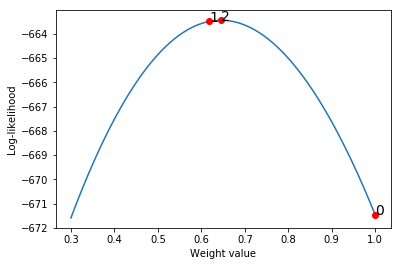
\includegraphics[scale=0.8]{Newton_method.png}
\end{figure}

The method saturates after two iterations. 

By visual inspection of the plots, it is clear that the algorithm finds the maximum likelihood value quite well. The goodness of the maximum likelihood value increases with increasing number of data points.  

\section{CASE 2}
 
The method was performed with various number of spike trains, $ \{1,10,100,1000,10000 \}$, and 3000 iterations of the algorithm was run for every instance. Figure \ref{fig:Case2_1} shows an example of normalized root mean squared errors over iterations for the different number of trials. Here the generative weight trajectory was the same for all the instances, and the initial guess was set to be the true weights. 


\begin{figure}[hbt!]
\caption{Normalized root MSE over iterations for various number of trials. One example of the method in case 2 when starting from the correct weights}
\label{fig:Case2_1}
    \centering
    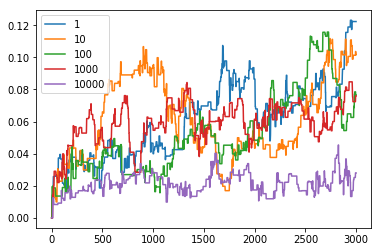
\includegraphics[scale=0.75]{MSE3.png}
\end{figure}

This procedure was repeated 100 times for each number of trials. The underlying weights were now drawn new for each replicate. Figure \ref{fig:case2_avg} shows the mean of the rnMSE values at each iteration, with variance bars around it. 

\begin{figure}[hbt!]
\caption{Average rnMSE with variance bars of 100 replicates for each number of trials. Initial guess set to the true weights.}
\label{fig:case2_avg}
    \centering
    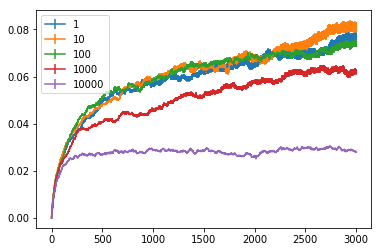
\includegraphics[scale=0.75]{Mean_plot_std.png}
\end{figure}

%\begin{figure}[hbt!]
    %\centering
    %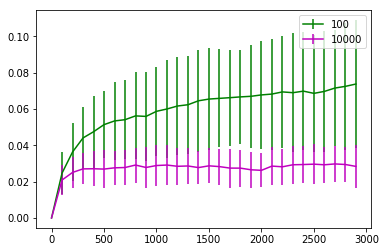
\includegraphics[scale=0.8]{Std_every100.png}
%\end{figure}


It is also interesting to see how well the algorithm manages to find the actual weights when the iterations begins from somewhere else. Now the initial guess for the MCMC iterations is set to be a random walk around 1. Figure \ref{fig:MSE2} shows the corresponding mean rnMSE of 100 replicates for each number of trials. 

%\begin{figure}[hbt!]
    %\centering
    %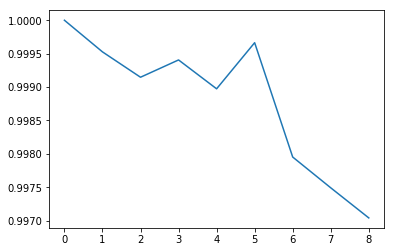
\includegraphics[scale=0.8]{Start_it_1000.png}
%\end{figure}


\begin{figure}[hbt!]
\caption{Average rnMSE with variance bars of 100 replicates for each number of trials. Initial guess set to random walk around 1}
\label{fig:MSE2}
    \centering
    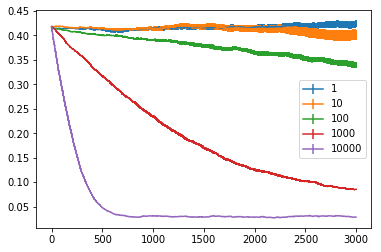
\includegraphics[scale=0.8]{MSE_starting_away.png}
\end{figure}

To visualize what is happening during the course of the iterations figure \ref{fig:trajectories} displays the how the estimated weights after 100,200,300,400,500 and 1000 iterations looks like, for initial guess a random walk around 1. 



\begin{figure}[hbt!]
\caption{Plots of the true weights (blue), the initial guess (orange), and the inferred weights after 100, 200, 300, 400, 500 and 1000 iterations (green)}
\label{fig:trajectories}
    \centering
    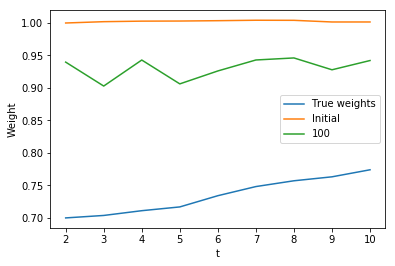
\includegraphics[scale=0.4]{fig/10000_100.png}
    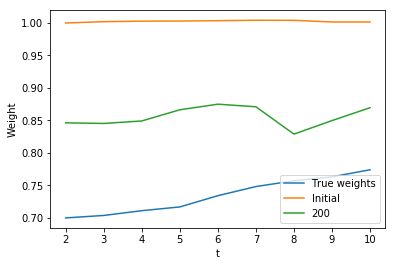
\includegraphics[scale = 0.4]{fig/10000_200.png}\\
    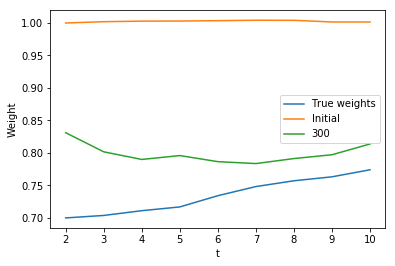
\includegraphics[scale = 0.4]{fig/10000_300.png}
    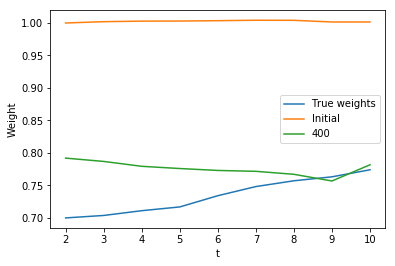
\includegraphics[scale = 0.4]{fig/10000_400.png}\\
    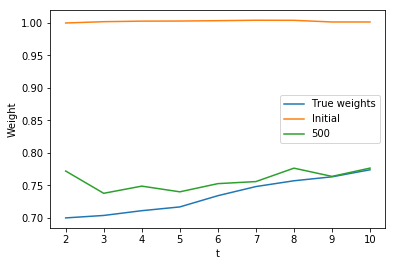
\includegraphics[scale = 0.4]{fig/10000_500.png}
    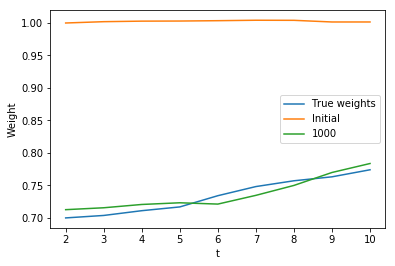
\includegraphics[scale = 0.4]{fig/10000_1000.png}
\end{figure}

\newpage

%\begin{figure}[hbt!]
    %\centering
    %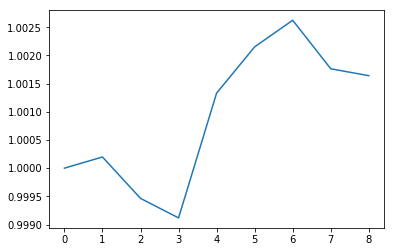
\includegraphics[scale=0.3]{fig/Start_it_100.png}
    %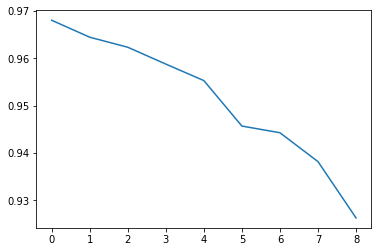
\includegraphics[scale = 0.3]{fig/1000_it_100.png}
    %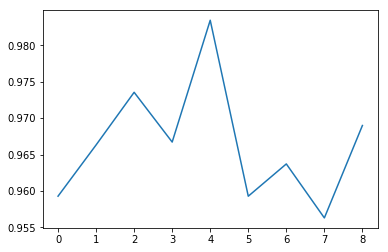
\includegraphics[scale = 0.3]{fig/2000_it_100.png}\\
    %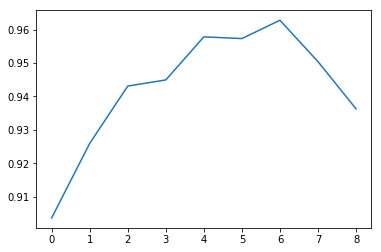
\includegraphics[scale = 0.3]{fig/3000_it_100.png}
    %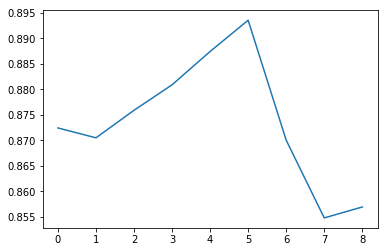
\includegraphics[scale = 0.3]{fig/4000_it_100.png}
    %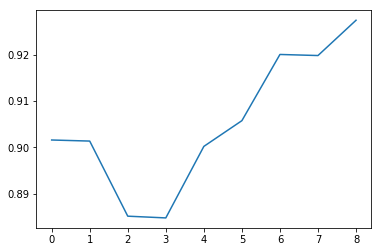
\includegraphics[scale = 0.3]{fig/5000_it_100.png}
    %\caption{Development of weight trajectory over iterations for 100 trials. 0, 1000, 2000, 3000, 4000 and 5000 iterations}
    %\label{w_trajectory_1000}
%\end{figure}

\section{CASE 3}
First the variant where the weight for all time steps are drawn individually were performed. This was tried with various values for the variance in the prior and proposal distribution. For a low value of the prior variance compared to the proposal variance, no new weight trajectories were accepted in the algorithm, so the estimation just stays where it starts. If the relative variance is large enough for weight trajectories to be accepted, it does not move towards the correct solution, and the error increases with iteration. One example of the true, initial and inferred weights after 3000 iterations is shown in figure \ref{fig:400_weights}. 


\begin{figure}
    \caption{True weights (orange), initial guess (green) and inferred weights (blue) after 3000 iterations}
    \label{fig:400_weights}
    \centering
    \includegraphics[scale=0.8]{fig/{Result_0.08}.png}
\end{figure}


Next, the same procedure was performed with dividing the time line into bins, and assuming constant weights within the bins. The initial guess was set to a random walk around 1. The result for dividing 300 seconds into 10 bins, and performing 3000 iterations is shown in figure \ref{fig:10bins}, with prior and proposal variance equal to 0.01, 0.005 and 0.0005.


\begin{figure}[hbt!]
\caption{True weights (orange), initial guess (green) and inferred weights (blue) for 10 bins and 3000 iterations. The prior and proposal distribution was 0.01 (top left), 0.005 (top right) and 0.0005 (bottom)}
\label{fig:10bins}
    \centering
    \includegraphics[scale=0.45]{fig/{10bins_0.01_0.01_s}.png}
    \includegraphics[scale=0.45]{fig/{10bins_0.005_0.005_s}.png}\\
    \includegraphics[scale=0.45]{fig/{10bins_0.0005_0.0005}.png}
\end{figure}

This was done for 1, 5, 10 and 20 number of bins, with 30 replicates for each. The mean of the rnMSE with variance bars for these are presented in figure \ref{fig:MSE_bins}. Here the prior and proposal variance used was 0.005, which was chosen as it gave reasonable results. 

\begin{figure}[hbt!]
\caption{}
\label{fig:MSE_bins}
    \centering
    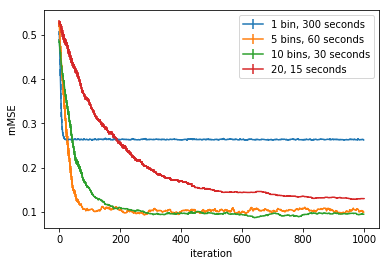
\includegraphics[scale=0.8]{fig/MSE_bins.png}
\end{figure}


\cleardoublepage